\chapter{Introduction}

  Depuis une dizaine d’années, les fabricants des processeurs haute-performance
  ont atteint des limitations physiques concernant la dissipation thermique et
  l'augmentation de la fréquence d'horloge. Ils se sont tournés vers les
  architectures multi-coeurs à mémoire partagée cohérente garantie par
  matériel. De nos jours, des processeurs à mémoire partagée cohérente ayant
  jusqu’à 100 coeurs intégrés sur la même puce sont une réalité et des
  processeurs multi-c\oe urs ayant plusieurs centaines, voire, un millier de
  coeurs sont à prévoir prochainement.
  
  Dans les architectures multi-c\oe urs à mémoire partagée cohérente, les coeurs
  sont typiquement regroupés dans des tuiles/clusters et le cache du dernier
  niveau est physiquement distribué sur ces derniers. Les tuiles/clusters sont
  reliés entre-eux par un NoC (Network-On-Chip). Par conséquent, la latence des
  accès mémoire liés aux miss des caches L1 est variable selon la distance
  séparant le coeurs demandeur du tuile/cluster contenant le cache L2
  responsable des lignes demandées. Dans ces architectures, la question de la
  localité du trafic généré par les miss de caches L1 (data, instruction et TLB)
  est primordiale à la fois pour passer à l’échelle et pour réduire la
  consommation électrique (énergie consommée par bit transféré).

  Pour répondre à cet enjeux de passage à l'échelle et de consommation
  énergétique, l'équipe ALSOC du LIP6 participe à deux projets d'envergures:
  SHARP~\cite{sharp2012} et TSAR~\cite{tsar2008}. Ce dernier a pour but de
  fournir une architecture matérielle passant à l'échelle de plusieurs centaines
  de coeurs, tandis que l'autre se veut être capable de fournir un système
  d'exploitation pour exploiter efficacement cette nouvelle architecture.

  Notre travail portera sur le multi-noyau ALMOS, et plus particulièrement sur
  la migration de tâches entre différentes instances du noyau. Nous allons dans
  un premier temps présenter l'architecture matérielle TSAR. L'étude de cette
  dernière est essentielle pour bien comprendre les enjeux d'ALMOS. Ensuite nous
  présenterons le noyau ALMOS, et notamment son cycle de vie, et enfin nous
  concluerons sur le travail que nous allons effectuer dans le cadre de ce
  stage.
  

  \section{L'architecture TSAR}

    TSAR est l'architecture d’un processeur multi-c\oe urs cc-NUMA homogène
    pouvant intégrer jusqu’à 4096 c\oe urs~\cite{greiner2009tsar}. Cette
    architecture est un résultat d’un projet de recherche européen
    MEDEA+~\cite{tsar2008} dont les principaux partenaires industriels sont
    BULL, Philips et THALES, et dont les partenaires académiques sont le LIP6 et
    le CEA-Leti. La figure \ref{fig:tsar} illustre un aperçu global de
    l'architecture TSAR. Il s'agit d'un ensemble de clusters interconnectés par
    un NoC (Network-On-Chip) DSPIN (Distributed, Scalable, Predictable,
    Integrated Network). Chaque c\oe ur dispose de ses propres caches L1 indexés
    en adresses physiques (données et instructions séparés) et d'une MMU (Memory
    Management Unit). La cohérence des caches de premier niveau de tous les c\oe
    urs ainsi que des TLBs est assurée par un protocole matériel nommé DHCCP
    (Distributed Hybrid Cache Coherence Protocol). Une description complète de
    cette architecture est disponible sur le site du projet
    TSAR~\cite{tsar2008web}.

    \begin{figure}[!h]
      \centering 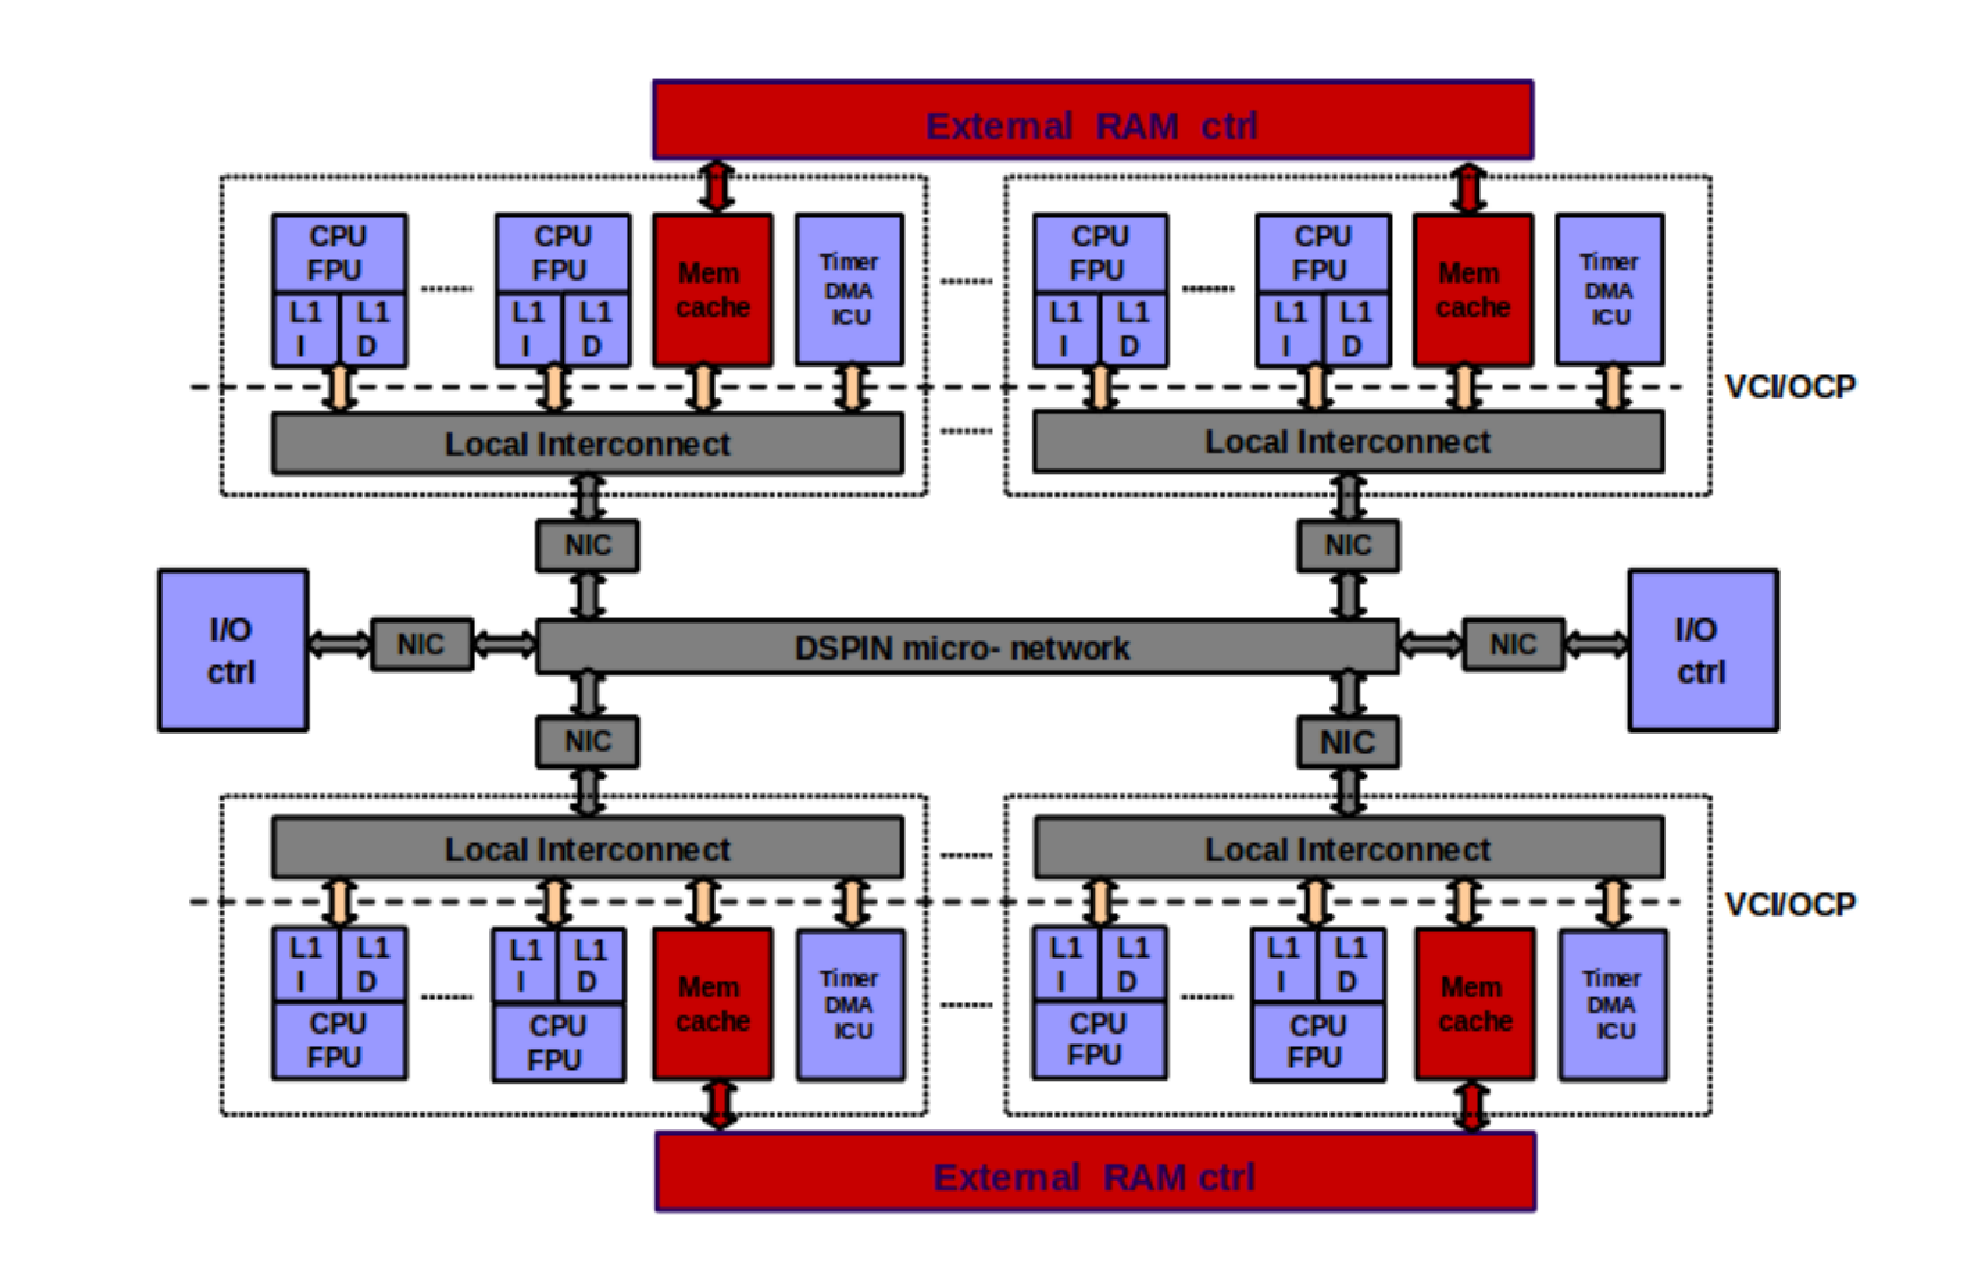
\includegraphics[scale=0.2]{include/img/tsar.png}
      \caption{Schéma global de l'architecture TSAR.~\cite{greiner2009tsar}}
      \label{fig:tsar}
    \end{figure}
  
  \section{Le noyau ALMOS}

    Le noyau ALMOS~\cite{almaless2011almos} est un noyau monolithique
    expérimental developpé au LIP6 par l'équipe ALSOC depuis 2011. Sujet de
    thèse de Ghassan Almaless, le développement est maintenant à la charge de
    Mohamed Karaoui (système de fichiers) et Clément Devigne (exécution de
    machines virtuelles). Le but d'ALMOS est de répondre à la problématique
    évoquée plus haut, à savoir la localité des accès mémoires dans les machines
    cc-NUMA. Une des particularité dans les choix architecturaux d'ALMOS est
    d'avoir choisit de développer un noyau monolithique.

    ALMOS est un noyau monolithique respectant la norme POSIX~\cite{posix2013}
    et implémentant différentes libraires: \texttt{libpthread, mpi,
      openMP}\ldots Le but premier d'ALMOS est de garantir un passage à
    l'échelle et une conservation de la localité des accès mémoires. Pour cela,
    le noyau intègre trois nouveaux mécanismes: \benumline \item les clusters
    managers \item les réplica-noyau \item une nouvelle stratégie d'allocation
    mémoire (Auto-Next-Touch) \eenumline.

    
    \subsection{Les cluster-manager}

      L'organisation distribuée du noyau d’ALMOS s’appuie sur les objets nommés
      gestionnaires de clusters (cluster-manager). L’objectif est d’une part, de
      décentraliser la gestion des ressources et d’autre part, d’assurer une
      localité d’accès mémoire lors de cette gestion. Un cluster-manager est un
      objet responsable de la gestion des ressources physiques (essentiellement
      c\oe urs et mémoire physique) d’un nœud cc-NUMA. Il existe autant de
      cluster-manager qu’il y a de clusters. Chacun de ces cluster-manager est
      placé localement dans la mémoire physique de son n\oe ud. Comme il est
      illustré par la figure ~\ref{fig:cluster_manager}, un cluster-manager
      contient, entre autres, un memory-manager et un ou plusieurs core-manager.
      Un core-manager est un objet responsable de la gestion d’un c\oe ur et
      plus précisément de l'ordonnancement des tâches affectées à ce c\oe urs
      ainsi que de la gestion des événements reçus par ce c\oe
      urs. L'ordonnancement est assuré par un serveur d'ordonnancement appelé
      (scheduler-server) tandis que la gestion des événements est assurée par un
      gestionnaire dédié (events-manager).

      \begin{figure}[!h]
        \centering 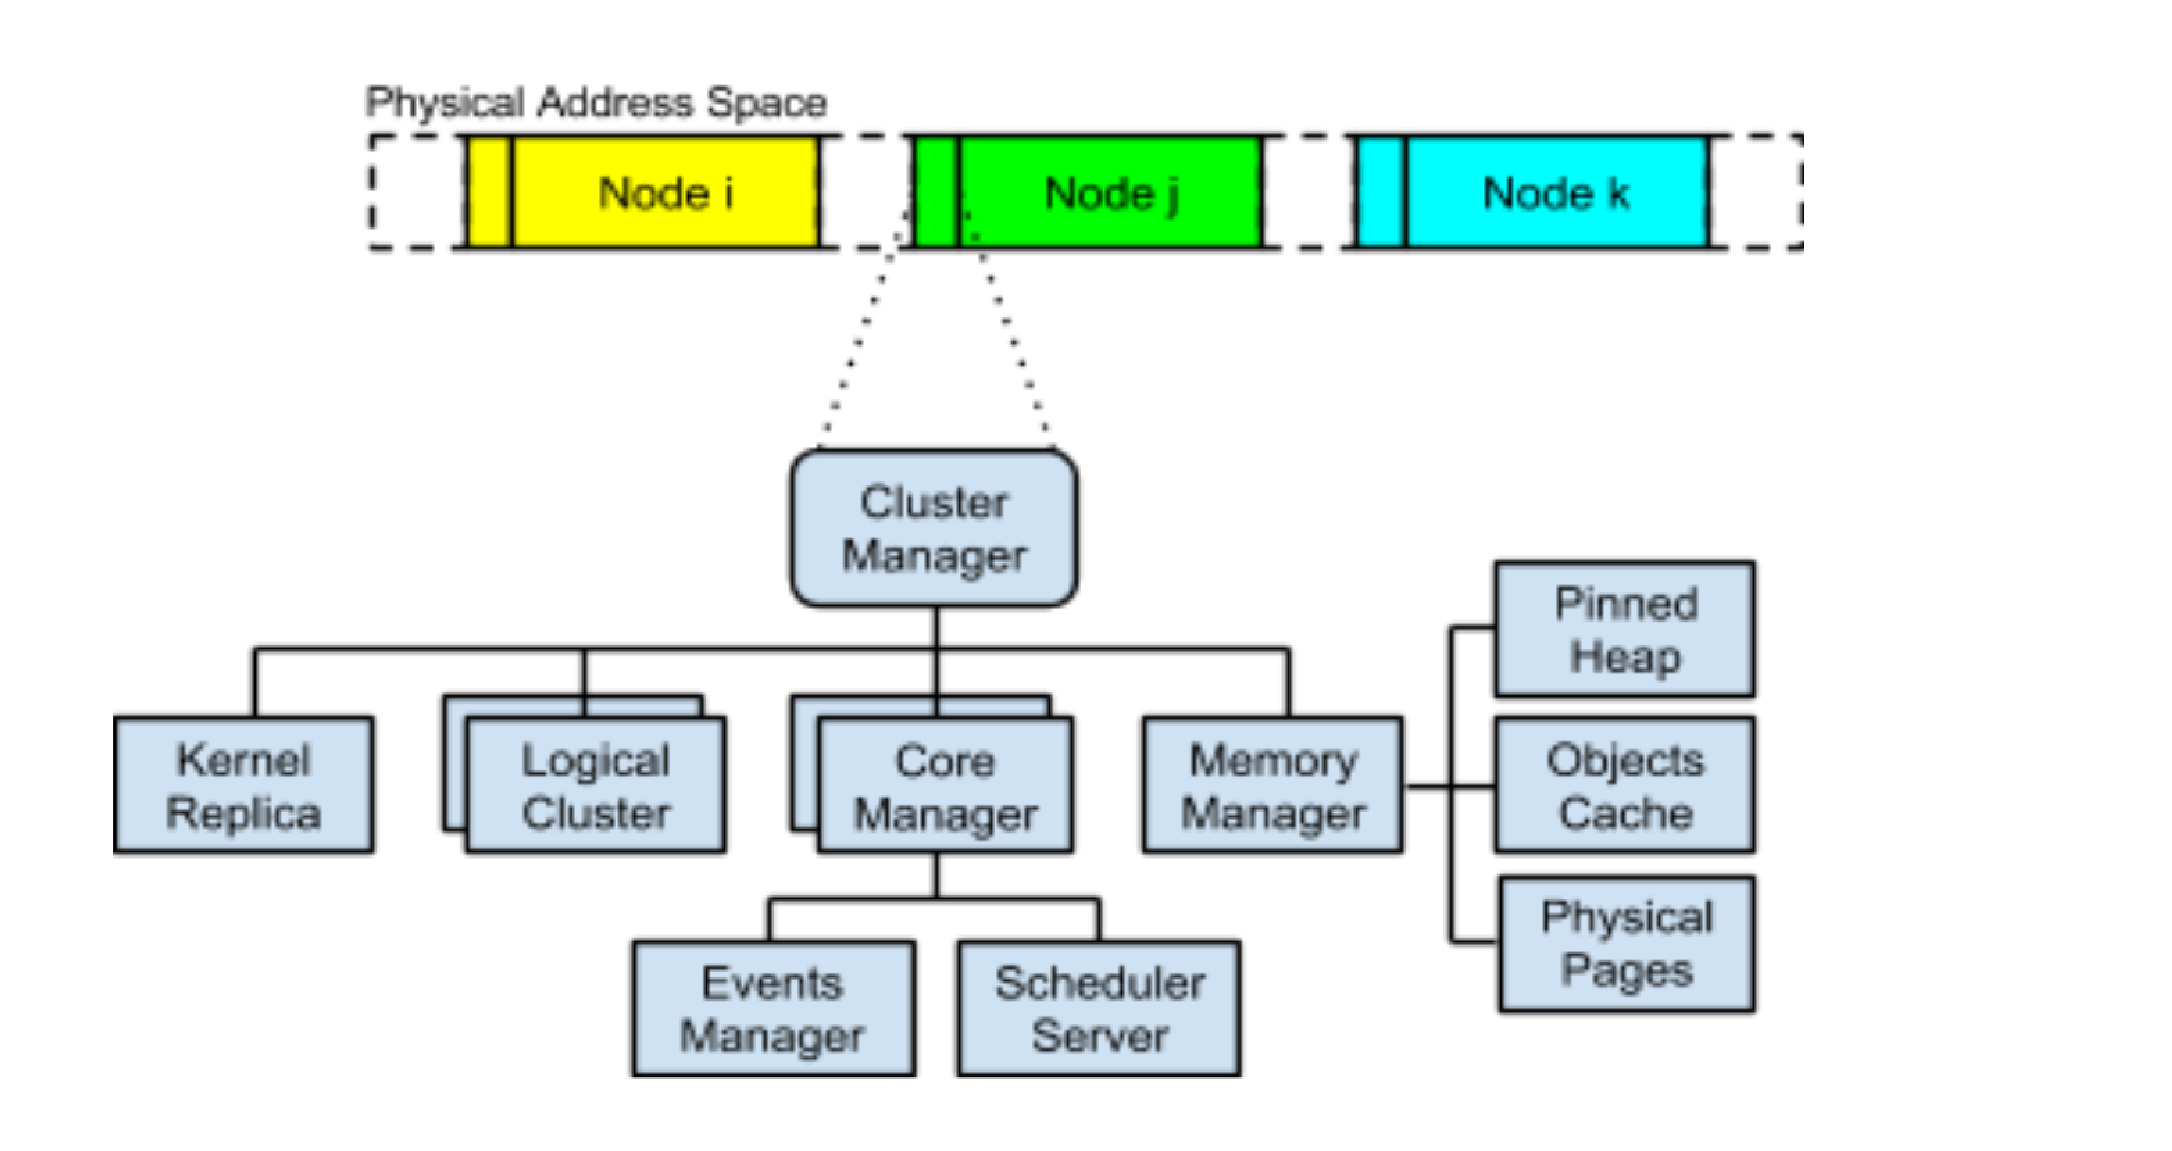
\includegraphics[scale=0.2]{include/img/cluster_manager}
        \caption{Un cluster manager est un gestionnaire de ressources d'un n\oe
          ud cc-NUMA. Il est physiquement placé dans le banc mémoire du n\oe ud
          correspondant.}
        \label{fig:cluster_manager}
      \end{figure}

      
    \subsection{Les réplica noyau}

      Comme nous l'avons vu précédemment, l'architecture TSAR offre au système
      d'exploitation la notion de cluster. Ces clusters sont ainsi composés de
      quatre processeurs\footnote{Dans la version TSAR-Leti} connectés entre eux
      sur un interonnect local, lui-même relié à différents périphériques (TTy,
      ICU, NIC, etc\ldots) (voir figure~\ref{fig:tsar_cluster}).
      
      \begin{figure}[!h]
        \centering 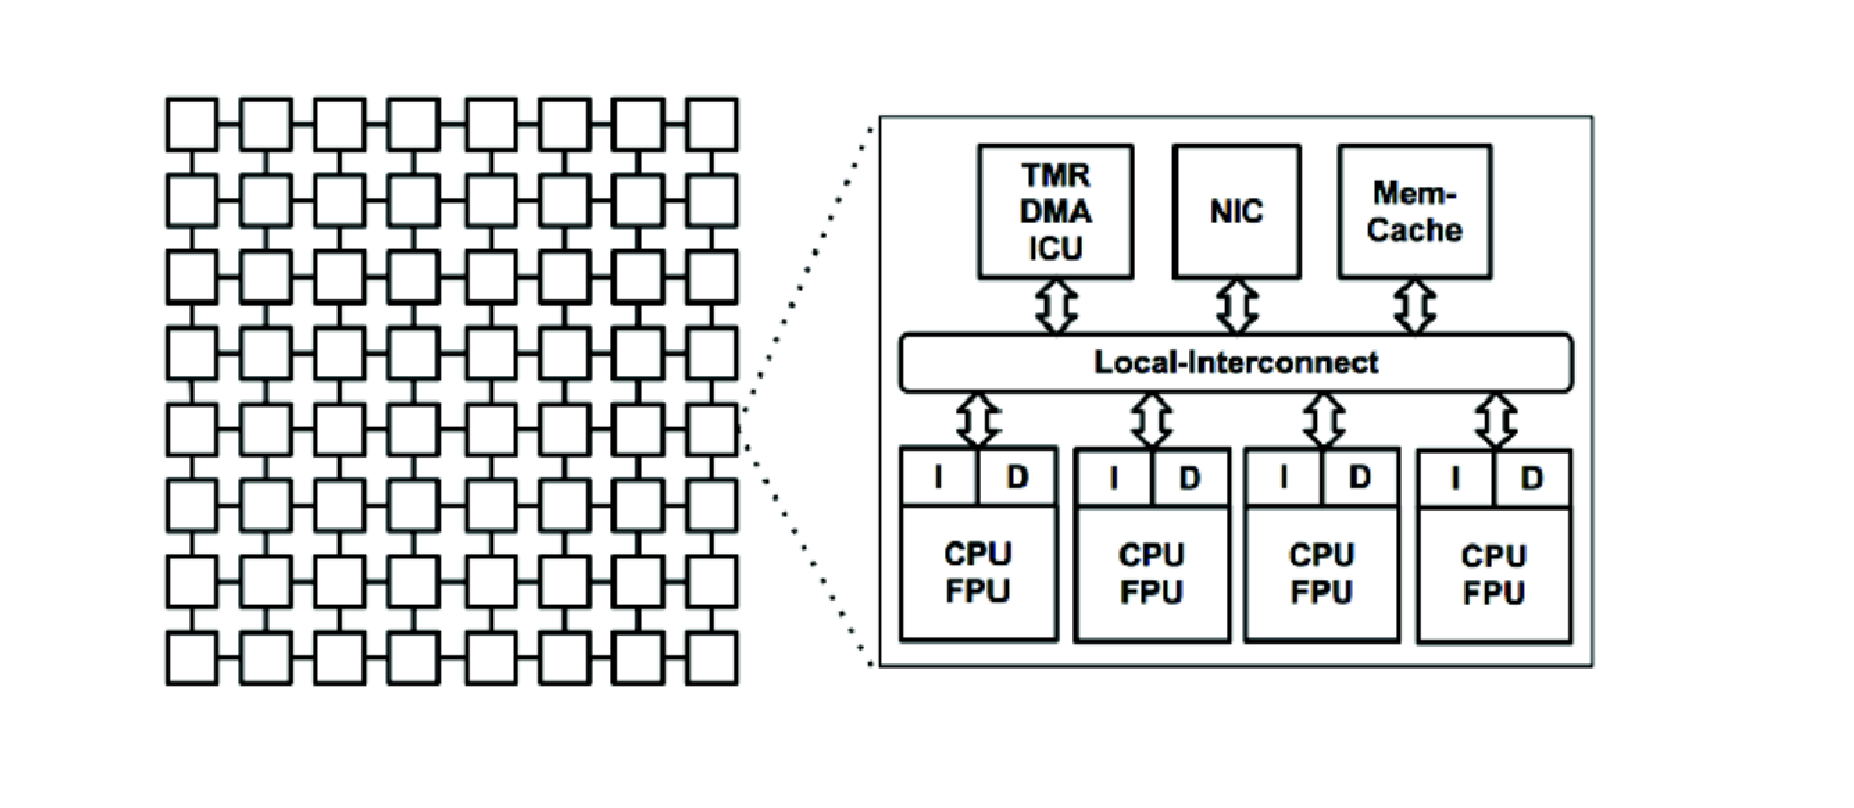
\includegraphics[scale=0.3]{include/img/tsar_clusters.png}
        \caption{Représentation de l'architecture TSAR avec un NoC 2D et un
          cluster~\cite{almaless2014universite}}
        \label{fig:tsar_cluster}

      \end{figure}

      La norme POSIX impose que dans espace d'adressage des processus, il y ait
      un espace représentant le noyau. Or, si le code et les données du noyau
      sont situés à un seul et unique endroit (le cluster 0 par exemple, celui
      utilisé au boot de la machine), alors on paiera le coût de l'architecture
      NUMA a chaque appel système, puisque l'on devra accéder à des pages
      distantes.

      Afin de résoudre ce problème, la notion de réplica noyau a été introduite
      au sein des clusters-manager. Un réplica noyau consiste à dupliquer le
      code du noyau et les données partagées dans les premières pages physiques
      de chaque cluster de l'architecture. Ces pages sont en lecture seule pour
      garantir la cohérence et la sécurité. Lors de la création d'un procesus
      sur un cluster, les pages de l'espace d'adressage du processus
      représentant le noyau correspondront aux pages physiques de son cluster.


  \section{\todo{L'allocation mémoire ?}}



  \section{Évolution du projet}

    \subsection{Limitations de la version initiale}
    \label{subsec:unsolved}
    
      Développé initialement pour une architecture 32 bits, le noyau ne peut pas
      supporter plus de 4Go de mémoire vive. Bien que TSAR allait évoluer vers
      une architecture 40 bits pour offrir 1 tera-octet de mémoire physique,
      l'objectif visé n'était pas de supporter une telle quantité de mémoire,
      mais bel et bien de supporter le passage à l'échelle de plusieurs
      centaines de coeurs. Ainsi, un des premiers problème d'ALMOS est le
      mapping de l'espace virtuel, qui se révèle être très naïf. En effet, lors
      de la phase de boot, ce dernier va chercher à mapper le maximum de la
      mémoire physique du cluster de boot dans son espace
      virtuel\footnote{Contraitement aux noyaux ``classiques'', ALMOS s'accordge
        2 giga-octet d'espace virtuel au lieu de 1.}. Donc, si ce cluster
      possède (au moins) 2Go de mémoire physique, l'ensemble du noyau est mappé
      dans ce seul cluster. De plus, cela ne laisse que 2Go de mémoire virtuelle
      pour les applications utilisateur. \todo{clarifier cette
        affirmation ? L'enlever ?}

      
    \subsection{Contributions de Francois Guerret}
      
      La gestion d'une telle quantité de mémoire fut le sujet de stage de
      Francois Guerret en 2014. Ce dernier
      proposa~\cite{guerret2014exploitation} différents changements pour ALMOS
      \benumline \item réduire l'espace virtuel noyau à 1Go \item répartir cet
      espace virtuel entre les clusters \item sortir de l'espace virtuel les
      structures de données du noyau de taille importante \eenumline. Ces
      changements sont représentés par la figure~\ref{fig:almos-guerret}

      \begin{paragraph}{Répartition de l'espace d'adressage noyau:}
        Elle est fonction du nombres de clusters de l'architecture
        ($\frac{\text{Taille virtuelle}}{\text{Nb clusters}}$). Pour une
        architecture TSAR-Leti 40 bits, on dipose de 256 clusters, on a donc
        $\frac{1000}{256}\approx4$Mo d'espace virtuel noyau par cluster.
      \end{paragraph}
      \begin{paragraph}{Gestion en adressage physiques de structures de données:}
        Avec 4Mo d'espace virtuel noyau par clusters, certaines structures de
        données ne pouvait plus être contenues dans un si petit espace. Dans un
        premier temps, la table des pages. Celle-ci, une fois pleine\footnote{Ce
          cas n'arrive jamais, mais il est néanmoins mathématiquement possible},
        peut atteindre une taille maximale de 8Mo\footnote{\todo{Expliquer cette
            valeur par la formule ?}}. De plus, chaque
        processus \footnote{\todo{Vérifier si la version d'ALMOS de Francois
            n'avait pas les processus hybrides, ce qui impliquerait que ce soit
            une table de pages par thread et pas par processus.}}  dipose de sa
        propre table de pages. Il est techniquement impossible de stocker 8Mo
        dans cet espace virtuel, Francois a donc choisi de sortir cette
        structure de l'espace virtuel.

        La seconde structure de donnée problématique est la table des
        descripteurs de pages physiques. En effet, la norme POSIX
        \footnote{\todo{Vérifier que c'est pas juste une convention de codage des
          noyaux}} impose de devoir décrire toutes les pages physiques qu'offre
        la mémoire. Ainsi, pour décrire le tera de mémoire offert par TSAR, il
        est nécessaire d'utiliser 14Go\footnote{\todo{Expliquer le calcul par la
            formule ?}} de mémoire, soit 56Mo par cluster. Une fois de plus, il
        est impossible de stocker cette structure dans l'espace virtuel
        noyau. Celle-ci a donc été sortie de l'espace d'adressage physique.
      \end{paragraph}

      \begin{figure}[!h]
        \centering
        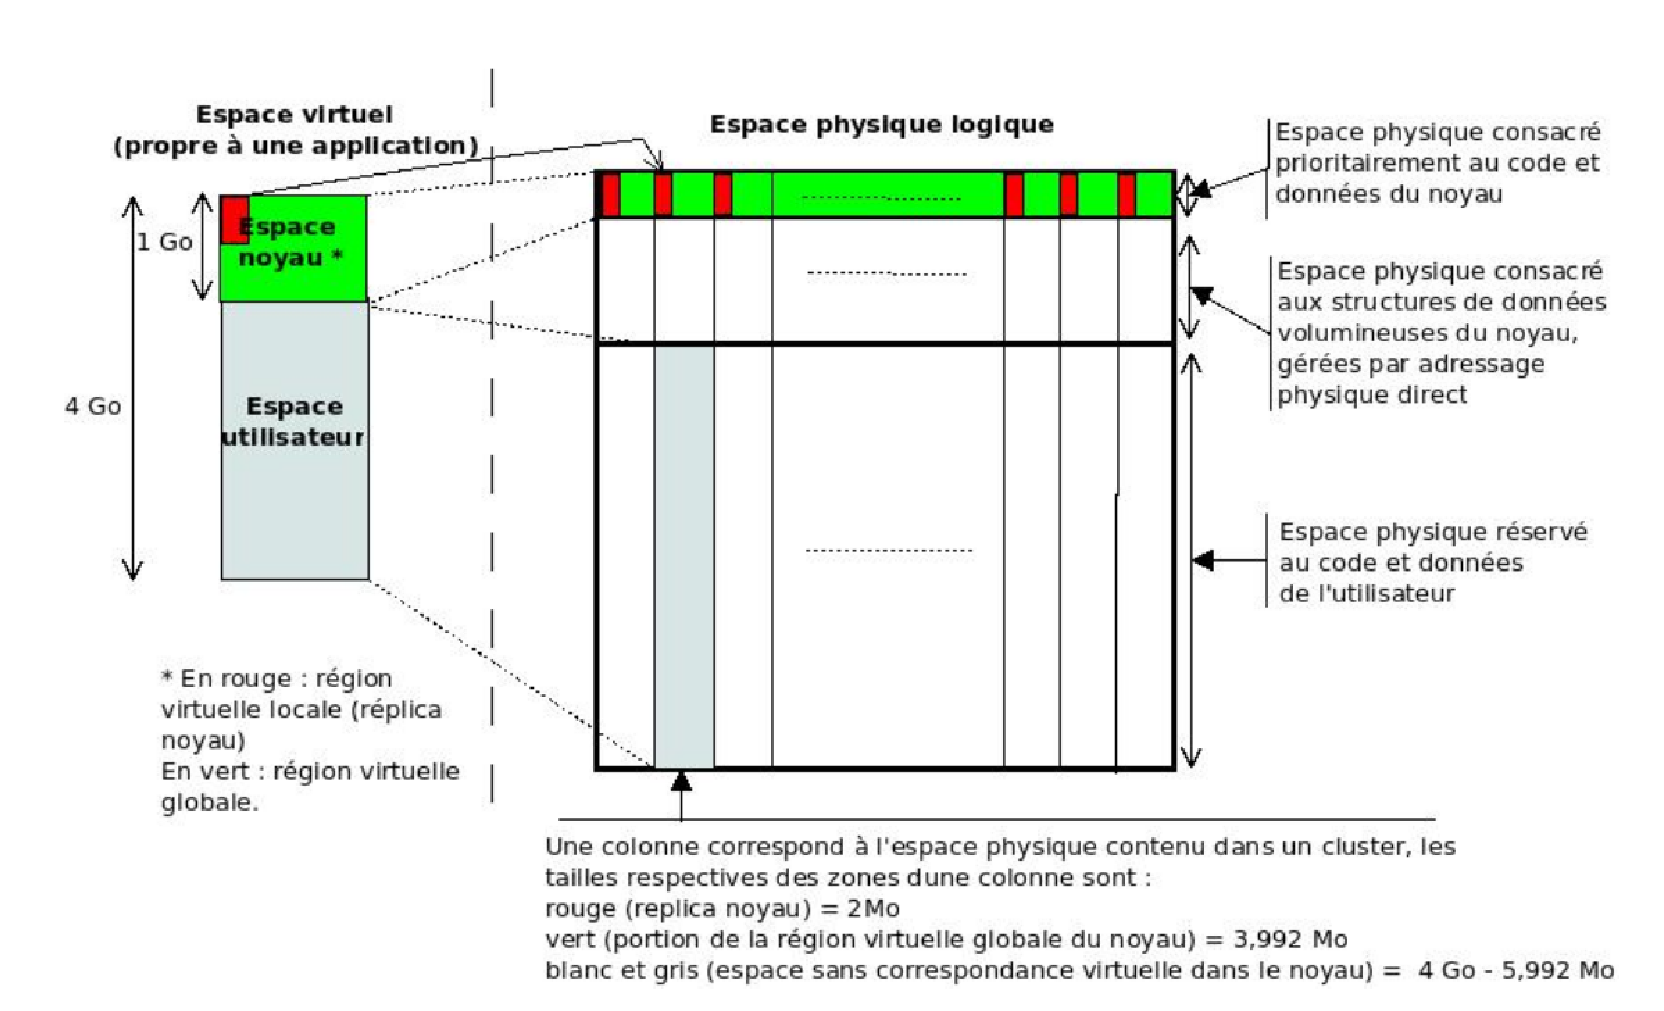
\includegraphics[scale=0.3]{include/img/almos-guerret}
        \caption{}
        \label{almos-guerret}
      \end{figure}
      
      \begin{paragraph}{Résultats:}
        Pour des raisons techniques\footnote{Sortir la tables de descripteurs de
          pages physiques du noyau nécessitait de recoder une grande partie du
          noyau)}, ce travail n'a malheureusement pas débouché sur une solution
        fonctionnelle, mais il a permis d'ouvrir la voie à la solution actuelle.
      \end{paragraph}

      
  \section{Passage au mode multi-noyau}
      
    La version actuelle de ALMOS proposée par Mohamed Karaoui et Franck Wajsbürt
    supprime totalement l'espace virtuel du noyau. Ce dernier fonctionne
    entièrement en adressage physique, et passe en mode multi-noyau, avec une
    instance de noyau dans chaque cluster. Ces changements \benumline \item
    permettent de gérer toute la mémoire physique de la plateforme TSAR, puisque
    chaque cluster dispose de 4Go de mémoire physique, et que l'on a un noyau
    par cluster \item permettent également de laisser 4Go de mémoire
    virtuelle\footnote{Modulo une page de petite taille (4Ko) pour faire le
      passage entre le mode utilisateur et le mode noyau} à
    l'utilisateur\eenumline.


    En revanche, l'inconvénient majeur apporté par cette solution est
    l'impossibilité d'accéder de manière directe à la mémoire des autres
    clusters. En effet, avec un noyau par cluster, les espaces d'adressage
    deviennent propres à ces derniers, et la vision d'un espace d'adressage
    unique entre les clusters n'existe plus. On ne peut donc plus accéder aux
    éléments des autres clusters de manière directe et transparente. Une des
    conséquences est d'avoir rendu non fonctionnelle la migration de
    processus/threads entre les clusters (la migration entre processeurs du même
    cluster est elle toujours fonctionnelle).

    \subsection{Traduction d'adresses}

      Si les processus utilisateurs utilisent toujours la mémoire virtuelle, ce
      n'est plus le cas du noyau. Nous allons voir comment celui-ci peut
      construire et manipuler des adresses sur 40 bits alors qu'il n'en dispoe
      que de 32 dans ses registres.

      \begin{paragraph}{Les processus utilisateurs:}
        Comme pour les autres noyaux, la traduction des adresses virtuelles en
        adresses physique sont faites par la MMU. Tout se processus est
        entièrement géré par le matériel. Le processeurs n'a pas conscience
        qu'il manipule des adresse virtuelles. Dans l'architecutre TSAR, la
        tables des pages est composées de deux niveaux d'indirections
        (figure~\ref{fig:page-table}).
        
        \begin{figure}
          \centering
          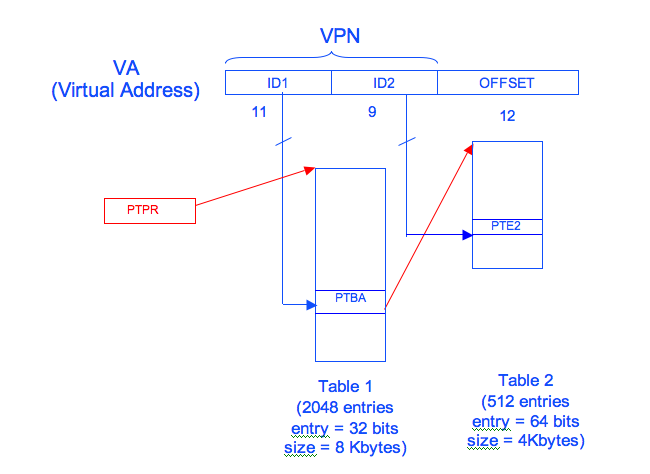
\includegraphics[scale=0.4]{include/img/pages_table_levels.png}
          \caption{La table des pages et sa hiérarchie (source: \textit{Greiner
              et al.}~\cite{tsar2008web})}
          \label{fig:page-table}
        \end{figure}
        
      \end{paragraph}
      \begin{paragraph}{Le noyau}
        Lors du passage en mode noyau, la MMU est désactivée. A partir de cet
        instant, toutes les adresses manipulées par le processeur seront des
        adresses physiques. Or, celles-ci sont sur 32 bits. Pour contourner
        cette limite, ALMOS exploite deux caractéristiques \benumline \item les
        processeurs récents disposent des registres d'extension d'adresses \item
        l'architecture clusterisé de TSAR numérote ces derniers par un système
        de coordonnées $cid = (x, y) | 0 \leq x,y \leq 255$ \eenumline. On va
        donc utiliser ces $x$ et $y$
      \end{paragraph}

      
  \section{Contributions}

    La problématique soulevée en~\ref{subsec:unsolved} est celle à laquelle nous
    allons répondre dans la suite de ce document. Plus précisément, il s'agit de
    définir et de mettre en place les mécanismes suivants:
    
    \begin{itemize}
      \item assurer la création et la migration de processus mono-threads entre
        clusters
      \item ajouter le support du multi-threading
      \item ré-implémenter le composant d'ALMOS appelé DQDT (Distributed
        Quaternary Decision Tree), assurant la vision globale de l'occupation
        des ressources matérielles de la plateforme, et par conséquent
        reponsable du placement des ressources sur celle-ci.
    \end{itemize}

    
    %% \subsection{Difficultés}

    %%   Le problème majeur de ces deux premiers objectifs est les structures de
    %%   données partagées entre des processus (notion de père/fils), ou des
    %%   threads d'un processus (l'esppace d'adressage du processus). Pour assurer
    %%   un service de migration, il faudra dupliquer ces structures, et assurer
    %%   \textbf{le maintient de la cohérence} entre elles. Le second problème est
    %%   la gestion d'un espage d'adressage physique plus grand que l'espace
    %%   virtuel du système. Ce sont ces deux axes de recherches qui seront
    %%   explorés dans le chapitre~\ref{chap:state-of-the-art}.
